\documentclass{article}
\usepackage{amsmath}
\usepackage{amssymb}
\usepackage{graphicx}
\usepackage{hyperref}
\usepackage[version=4]{mhchem}

\title{Problem 11}
\date{}

\begin{document}
\maketitle

\section*{Problem}
Prove the Angle Bisector Theorem: The angle bisector of a triangle divides the opposite side into segments that are proportional to the adjacent sides.\\
\(\frac{A B}{A C}=\frac{B D}{C D} \quad\) or \(\quad \frac{A B}{B D}=\frac{A C}{C D}\)\\
\centering
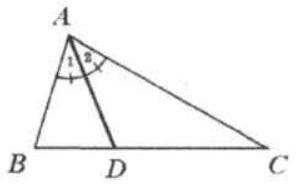
\includegraphics[width=\textwidth]{images/128(2).jpg}

\section*{Solution}
Solution not available.

\end{document}
